% DMXpress — The Console Upgrade
% A visual before/after guide. Build with: tectonic DMXpress-Guide.tex
\documentclass[11pt]{article}

\usepackage[a4paper,margin=2cm]{geometry}
\usepackage[table,svgnames]{xcolor}
\usepackage{tikz}
\usetikzlibrary{arrows.meta,positioning,calc,shapes.geometric,backgrounds,fit,decorations.pathreplacing}
\usepackage[most]{tcolorbox}
\usepackage{titlesec}
\usepackage{enumitem}
\usepackage{booktabs}
\usepackage{array}
\usepackage{tabularx}
\usepackage{hyperref}

% ---- palette -------------------------------------------------------------
\definecolor{ink}{HTML}{151A2B}
\definecolor{panel}{HTML}{222C49}
\definecolor{accent}{HTML}{18A999}
\definecolor{gold}{HTML}{E0A82E}
\definecolor{cred}{HTML}{E0524E}
\definecolor{cgreen}{HTML}{3FB36B}
\definecolor{cblue}{HTML}{3D7BE0}
\definecolor{cmag}{HTML}{C44FC4}
\definecolor{cgray}{HTML}{8A93A6}
\definecolor{line}{HTML}{C7CEDC}

\hypersetup{colorlinks=true, linkcolor=accent, urlcolor=accent, pdftitle={DMXpress — The Console Upgrade}}

% ---- type / layout -------------------------------------------------------
\setlength{\parindent}{0pt}
\setlength{\parskip}{5pt}
\setlist{itemsep=2pt, topsep=3pt, leftmargin=1.4em}

\titleformat{\section}{\Large\bfseries\color{ink}}{\thesection}{0.6em}{}[{\color{accent}\titlerule[1.2pt]}]
\titleformat{\subsection}{\large\bfseries\color{accent!70!ink}}{\thesubsection}{0.5em}{}
\titlespacing*{\section}{0pt}{16pt}{6pt}

% ---- tikz styles ---------------------------------------------------------
\tikzset{
  box/.style={rounded corners=3pt, draw=line, line width=0.9pt, fill=white, inner sep=7pt, font=\small, align=center},
  darkbox/.style={rounded corners=4pt, draw=none, fill=panel, text=white, inner sep=9pt, font=\small\bfseries, align=center},
  pool/.style={rounded corners=3pt, draw=accent, line width=1pt, fill=accent!10, inner sep=6pt, font=\small\bfseries, text=ink, align=center, minimum width=2.4cm},
  flow/.style={-{Latex[length=2.4mm]}, line width=1pt, draw=cgray},
  flowd/.style={-{Latex[length=2.4mm]}, line width=1pt, draw=cred, dashed},
}

% ---- tcolorboxes ---------------------------------------------------------
\newtcolorbox{concept}[1][The idea]{colback=accent!7,colframe=accent,coltitle=white,colbacktitle=accent,fonttitle=\bfseries,title=#1,arc=3pt,boxrule=0.9pt,left=8pt,right=8pt}
\newtcolorbox{tipbox}[1][Tip]{colback=cgreen!8,colframe=cgreen,coltitle=white,colbacktitle=cgreen,fonttitle=\bfseries,title=#1,arc=3pt,boxrule=0.9pt,left=8pt,right=8pt}
\newtcolorbox{gotcha}[1][Watch out]{colback=cred!7,colframe=cred,coltitle=white,colbacktitle=cred,fonttitle=\bfseries,title=#1,arc=3pt,boxrule=0.9pt,left=8pt,right=8pt}

% toolbar-style badge (replaces the app's emoji labels)
\newcommand{\badge}[2]{\tikz[baseline=(b.base)]{\node[fill=#1,rounded corners=2.5pt,inner xsep=5pt,inner ysep=1.6pt,text=white,font=\footnotesize\bfseries](b){#2};}}

\newcommand{\then}{\textcolor{cgray}{\textbf{THEN}}}
\newcommand{\now}{\textcolor{accent}{\textbf{NOW}}}
\newcolumntype{Y}{>{\raggedright\arraybackslash}X}
\newcommand{\hd}[1]{\textbf{\textcolor{white}{#1}}}

% =========================================================================
\begin{document}

% ---- TITLE PAGE ----------------------------------------------------------
\begin{titlepage}
\centering
\vspace*{1.4cm}
{\fontsize{40}{44}\selectfont\bfseries\color{ink}DMXpress}\\[4pt]
{\Large\bfseries\color{accent}The Console Upgrade}\\[10pt]
{\large\color{cgray}How it used to work — and how it works now}\\[1.2cm]

% --- decorative fader bank ---
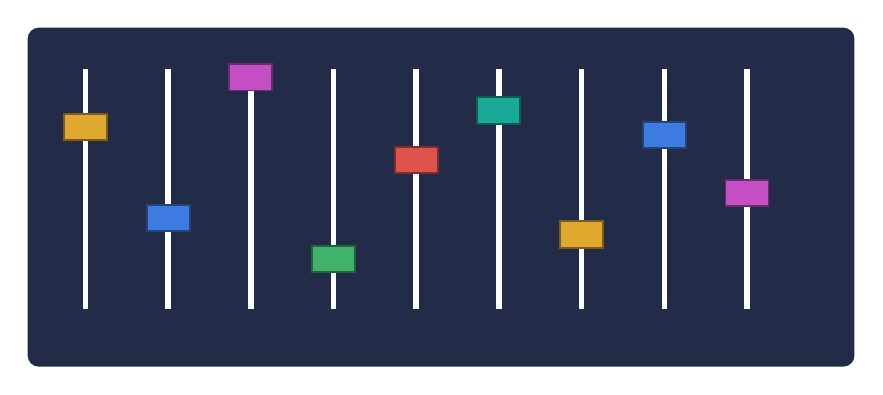
\begin{tikzpicture}[scale=1.05]
  \fill[panel,rounded corners=4pt] (-0.7,-0.6) rectangle (9.3,3.5);
  \foreach \i/\h/\c in {0/2.3/gold,1/1.2/cblue,2/2.9/cmag,3/0.7/cgreen,4/1.9/cred,5/2.5/accent,6/1.0/gold,7/2.2/cblue,8/1.5/cmag}{
    \begin{scope}[xshift=\i cm]
      \draw[line width=2pt, color=white!22] (0,0.1) -- (0,3.0);
      \fill[\c] (-0.26,\h-0.16) rectangle (0.26,\h+0.16);
      \draw[\c!55!black, line width=0.7pt] (-0.26,\h-0.16) rectangle (0.26,\h+0.16);
    \end{scope}
  }
\end{tikzpicture}\\[1.2cm]

{\large\color{ink}From a one-look DMX tool $\;\longrightarrow\;$ a grandMA3-style lighting console}\\[6pt]
{\color{cgray}\small A visual companion to \texttt{GUIDE.md} \;\textbullet\; \today}
\end{titlepage}

% ---- AT A GLANCE ---------------------------------------------------------
\section*{What changed, in one breath}
\addcontentsline{toc}{section}{What changed}

DMXpress began as a simple controller: you picked a fixture, dragged some
sliders, and whatever you were touching went straight out the door. It is now a
small \emph{console} — with reusable selections, referenced presets, effects,
recorded cue lists, and a fader bank — built around one professional idea: a
\textbf{Programmer} that always sits on top of your \textbf{Playback}.

\begin{center}\small
\rowcolors{2}{accent!5}{white}
\begin{tabularx}{\linewidth}{>{\bfseries}l Y Y}
\arrayrulecolor{accent}\toprule
\rowcolor{ink}\hd{Area} & \hd{Then} & \hd{Now}\\
\midrule
Output model      & One live look straight to DMX            & Mixer of layers, Programmer on top\\
Selecting         & Click a fixture                          & Click \emph{+} reusable \badge{cmag}{Groups}\\
Storing looks     & ShowBuddy presets (read-only)            & \badge{cmag}{Palettes} per feature (your own)\\
Effects           & \badge{cmag}{Chases} (one moving preset) & \badge{cmag}{Phasers} across a selection\\
Playback          & \badge{cmag}{Transition} crossfade       & \badge{cmag}{Stacks} (tracking cues) + \badge{cmag}{Decks}\\
Master            & ---                                      & Grand Master + per-stack faders\\
Operating         & Mouse only                               & \badge{cmag}{Command} line + \badge{cmag}{Views}\\
\bottomrule
\end{tabularx}
\end{center}

% ---- THE BIG SHIFT -------------------------------------------------------
\section{The big shift: one look becomes a console}

\subsection{\then\;\; the old signal flow}
Everything funnelled into a single \texttt{Look}. Editing a channel \emph{was}
the show; there was nowhere to \emph{store} your own looks and nothing playing
underneath.

\begin{center}
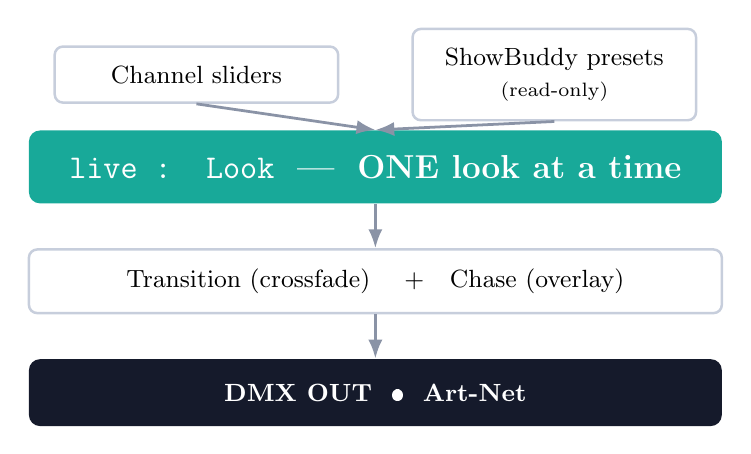
\begin{tikzpicture}[node distance=16pt]
  \node[box,minimum width=3.6cm](cs){Channel sliders};
  \node[box,minimum width=3.6cm,right=26pt of cs](pr){ShowBuddy presets\\ \scriptsize(read-only)};
  \node[darkbox,fill=accent,minimum width=8.8cm,below=20pt of $(cs)!0.5!(pr)$](look){\large \texttt{live : Look} \;---\; ONE look at a time};
  \node[box,minimum width=8.8cm,below=16pt of look](tr){Transition (crossfade) \quad+\quad Chase (overlay)};
  \node[darkbox,fill=ink,minimum width=8.8cm,below=16pt of tr](dmx){DMX OUT \;\textbullet\; Art-Net};
  \draw[flow](cs.south)--(look.north);
  \draw[flow](pr.south)--(look.north);
  \draw[flow](look)--(tr);
  \draw[flow](tr)--(dmx);
\end{tikzpicture}
\end{center}
\begin{center}\small\color{cgray}
No stored Groups, Palettes, or Cues. No faders. Whatever you edit is the output.
\end{center}

\subsection{\now\;\; the console pipeline}
The pools (Groups, Palettes, Phasers) feed a \textbf{Programmer}. The Programmer
overlays \emph{only the channels you touched} on top of a \textbf{Mixer} of
playing Stacks. \textbf{Store} records the Programmer down into a cue; a
\textbf{Grand Master} trims the whole rig on the way out.

\begin{center}
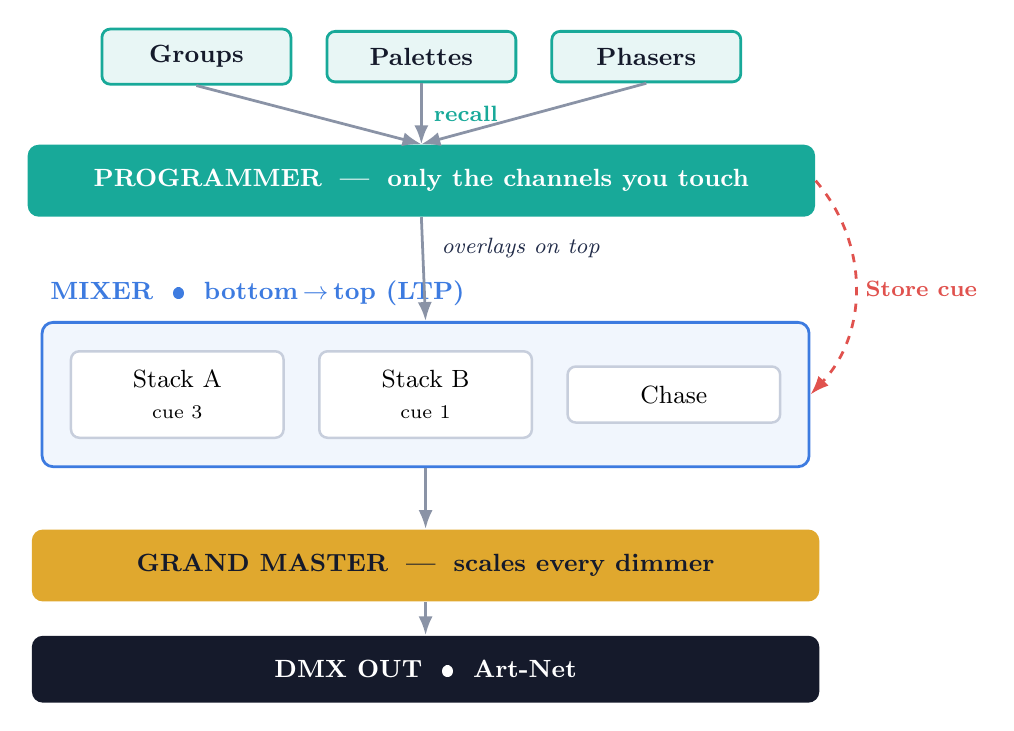
\begin{tikzpicture}[node distance=12pt and 12pt]
  % pools
  \node[pool](g){Groups};
  \node[pool,right=of g](p){Palettes};
  \node[pool,right=of p](ph){Phasers};
  % programmer
  \node[darkbox,fill=accent,minimum width=10cm,below=22pt of p](prog){PROGRAMMER \;---\; only the channels you touch};
  % mixer
  \node[box,minimum width=2.7cm,below=48pt of prog,xshift=-3.1cm](sa){Stack A\\\scriptsize cue 3};
  \node[box,minimum width=2.7cm,right=12pt of sa](sb){Stack B\\\scriptsize cue 1};
  \node[box,minimum width=2.7cm,right=12pt of sb](ch){Chase};
  \begin{scope}[on background layer]
    \node[draw=cblue,line width=1pt,rounded corners=4pt,fill=cblue!7,fit=(sa)(sb)(ch),inner sep=10pt](mix){};
  \end{scope}
  \node[cblue,font=\small\bfseries,anchor=south west] at ([yshift=2pt]mix.north west){MIXER \;\textbullet\; bottom\,$\to$\,top (LTP)};
  % master + out
  \node[darkbox,fill=gold,text=ink,minimum width=10cm,below=22pt of mix](gm){GRAND MASTER \;---\; scales every dimmer};
  \node[darkbox,fill=ink,minimum width=10cm,below=12pt of gm](dmx){DMX OUT \;\textbullet\; Art-Net};
  % arrows
  \draw[flow](g.south)--(prog.north);
  \draw[flow](p.south)--(prog.north);
  \draw[flow](ph.south)--(prog.north);
  \node[font=\footnotesize\bfseries,text=accent,right=1pt] at ($(p.south)!0.5!(prog.north)$){recall};
  \draw[flow](prog.south)--(mix.north) node[pos=0.3,right=3pt,font=\footnotesize\itshape,text=panel]{overlays on top};
  \draw[flowd](prog.east) to[bend left=42] node[right,font=\footnotesize\bfseries,text=cred]{Store cue} (mix.east);
  \draw[flow](mix.south)--(gm.north);
  \draw[flow](gm.south)--(dmx.north);
\end{tikzpicture}
\end{center}

% ---- MENTAL MODEL --------------------------------------------------------
\section{The mental model: Programmer on top of Playback}

\begin{concept}
You \textbf{build} a look in the \textbf{Programmer} (your scratch pad), then
\textbf{Store} it into something reusable. Playback (Stacks/Decks) runs
\emph{underneath} the Programmer, so whatever you are editing always wins ---
until you \textbf{Clear}.
\end{concept}

The Programmer only asserts the channels you have touched since the last Clear.
Below, two Stacks are playing; you are editing channels 4--7, so the Programmer
overrides exactly those and the rest of the show tracks through untouched.

\begin{center}
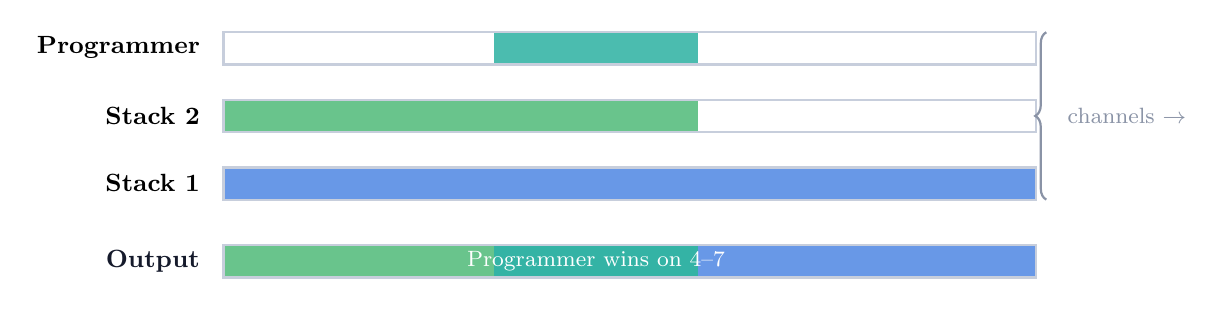
\begin{tikzpicture}[x=0.86cm,y=0.66cm]
  \foreach \y/\name/\col/\a/\b in {2.6/{Programmer}/accent/4/7, 1.3/{Stack 2}/cgreen/0/7, 0/{Stack 1}/cblue/0/12}{
    \node[left=5pt,font=\small\bfseries] at (0,\y+0.32){\name};
    \fill[\col!78] (\a,\y) rectangle (\b,\y+0.62);
    \draw[line,line width=0.8pt] (0,\y) rectangle (12,\y+0.62);
  }
  % result lane
  \node[left=5pt,font=\small\bfseries,text=ink] at (0,-1.5+0.32){Output};
  \fill[cblue!78](0,-1.5) rectangle (12,-0.88);
  \fill[cgreen!78](0,-1.5) rectangle (7,-0.88);
  \fill[accent!88](4,-1.5) rectangle (7,-0.88);
  \draw[line,line width=0.8pt](0,-1.5) rectangle (12,-0.88);
  \node[font=\footnotesize,text=white] at (5.5,-1.19){Programmer wins on 4--7};
  \draw[decorate,decoration={brace,amplitude=4pt},line width=0.8pt,cgray] (12.15,0) -- node[right=4pt,font=\footnotesize,text=cgray]{channels $\to$} (12.15,3.22);
\end{tikzpicture}
\end{center}

\begin{gotcha}[The \#1 newcomer trap]
If your faders and \textbf{Go} button ``do nothing'', the Programmer is still
holding those channels. Press \textbf{Clear prog} (or type \texttt{clear}) to
release it so your Stacks and Decks take over the output.
\end{gotcha}

% ---- THE SCREEN ----------------------------------------------------------
\section{The screen now}

\begin{center}
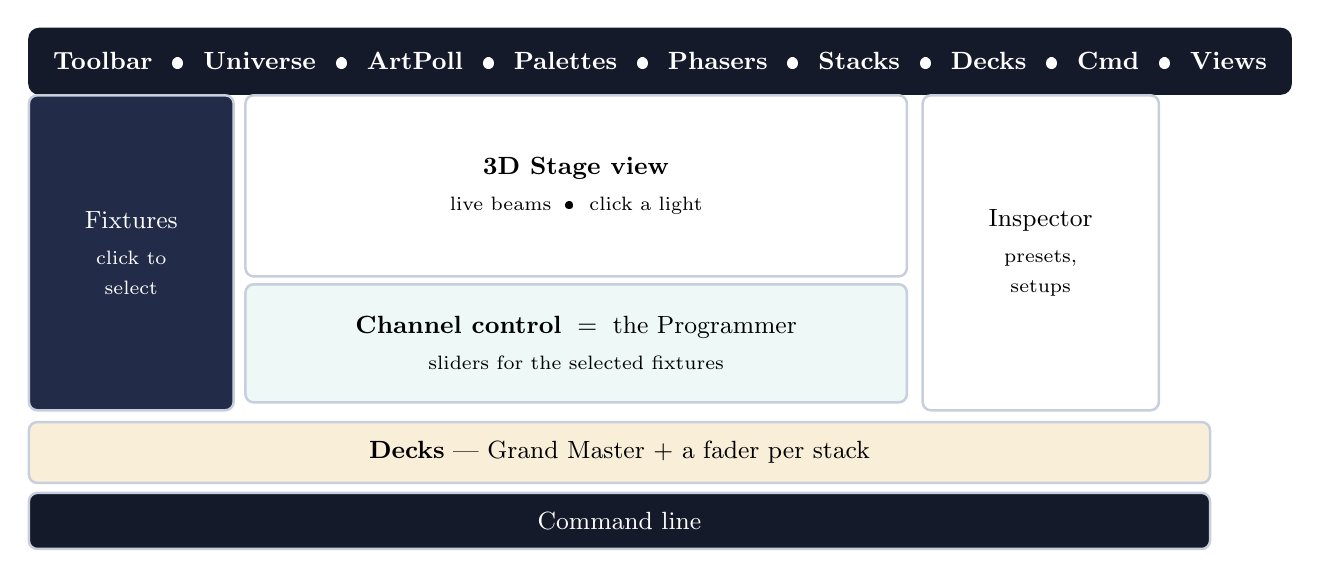
\begin{tikzpicture}[font=\small]
  % toolbar
  \node[darkbox,fill=ink,minimum width=15cm,minimum height=0.7cm,anchor=north west](tb) at (0,0){Toolbar \;\textbullet\; Universe \;\textbullet\; ArtPoll \;\textbullet\; Palettes \;\textbullet\; Phasers \;\textbullet\; Stacks \;\textbullet\; Decks \;\textbullet\; Cmd \;\textbullet\; Views};
  % left
  \node[box,fill=panel,text=white,minimum width=2.6cm,minimum height=4.0cm,anchor=north west,align=center](fx) at (0,-0.85){Fixtures\\[2pt]\scriptsize click to\\ \scriptsize select};
  % center stage
  \node[box,minimum width=8.4cm,minimum height=2.3cm,anchor=north west,align=center](st) at (2.75,-0.85){\textbf{3D Stage view}\\[2pt]\scriptsize live beams \;\textbullet\; click a light};
  % center channel control
  \node[box,fill=accent!8,minimum width=8.4cm,minimum height=1.5cm,anchor=north west,align=center](cc) at (2.75,-3.25){\textbf{Channel control} \;=\; the Programmer\\[2pt]\scriptsize sliders for the selected fixtures};
  % right inspector
  \node[box,minimum width=3.0cm,minimum height=4.0cm,anchor=north west,align=center](ins) at (11.35,-0.85){Inspector\\[2pt]\scriptsize presets,\\ \scriptsize setups};
  % decks
  \node[box,fill=gold!18,minimum width=15cm,minimum height=0.75cm,anchor=north west,align=center](dk) at (0,-5.0){\textbf{Decks} --- Grand Master + a fader per stack};
  % command
  \node[box,fill=ink,text=white,minimum width=15cm,minimum height=0.6cm,anchor=north west,align=center](cmd) at (0,-5.9){Command line};
\end{tikzpicture}
\end{center}
\begin{center}\small\color{cgray}
Floating pools (Palettes, Phasers, Stacks, Groups, Views) open on top from the toolbar. Every panel has its own zoom control.
\end{center}

% ---- FEATURE BY FEATURE --------------------------------------------------
\section{Then vs Now, feature by feature}

\subsection{Selecting \& setting values}
\begin{tabularx}{\linewidth}{p{2.3cm} Y Y}
\arrayrulecolor{line}\toprule
& \then & \now\\
\midrule
Selection & Click one fixture at a time. & Click, \textbf{Shift}-click to add/remove, \textbf{Cmd}-click for same type --- and save selections as \badge{cmag}{Groups}.\\
Values & Drag channel sliders; that is the output. & Same sliders, but every channel you touch joins the \textbf{Programmer} (an overlay you can store or clear).\\
\bottomrule
\end{tabularx}

\subsection{Storing looks: Palettes (the big new idea)}
\begin{concept}[Why Palettes change everything]
A \textbf{Palette} stores a value for \emph{one feature} --- Color, Position,
Dimmer, Beam, Focus, or Control. Recall ``Blue'' without moving the lights;
recall ``Center'' without changing their color. Cues remember the \emph{palette
reference}, so re-tinting ``Blue'' updates every cue that used it.
\end{concept}

The six feature pools, each its own tab in the Palettes window:
\begin{center}
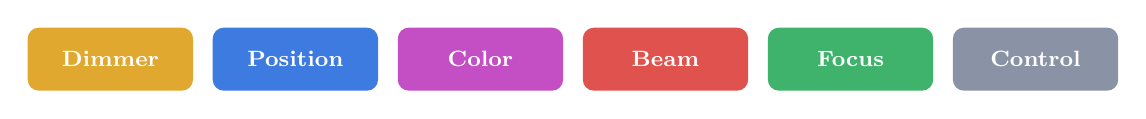
\begin{tikzpicture}[font=\footnotesize\bfseries]
  \foreach \i/\name/\c in {0/Dimmer/gold,1/Position/cblue,2/Color/cmag,3/Beam/cred,4/Focus/cgreen,5/Control/cgray}{
    \node[rounded corners=4pt,fill=\c,text=white,minimum width=2.1cm,minimum height=0.8cm] at (\i*2.35,0){\name};
  }
\end{tikzpicture}
\end{center}
\begin{center}\small\color{cgray}
\then\; ShowBuddy presets were whole-rig and read-only. \quad \now\; you build your own, per feature, and reference them in cues.
\end{center}

\subsection{Effects: Chases became Phasers}
\begin{tabularx}{\linewidth}{p{2.3cm} Y Y}
\arrayrulecolor{line}\toprule
& \then & \now\\
\midrule
Movement & A \textbf{Chase} swept one preset around a circle. & A \textbf{Phaser} drives any feature across your selection --- sine, chase, rainbow, sweep --- with \emph{Spread} and \emph{Wings}.\\
Reuse & Configured live, not stored. & Stored as tiles; click to re-apply, and they record into cues.\\
\bottomrule
\end{tabularx}

\subsection{Playback: from a crossfade to cue stacks + faders}
\begin{tabularx}{\linewidth}{p{2.3cm} Y Y}
\arrayrulecolor{line}\toprule
& \then & \now\\
\midrule
Looks over time & One \textbf{Transition} crossfaded between looks. & A \textbf{Stack} is an ordered cue list; \textbf{Go} fades to the next cue. Untouched channels \emph{track} through.\\
Surface & --- & The \textbf{Decks} bar: a Grand Master plus a level fader, \textbf{Go} and \textbf{Off} per stack.\\
\bottomrule
\end{tabularx}

\subsection{Operating: mouse, plus a command line and Views}
\then\; everything was clicks. \quad \now\; type \texttt{clear}, \texttt{go},
\texttt{store}, \texttt{cue 3}, \texttt{group 1}, \texttt{gm 80} on the
\badge{cmag}{Command} line, and snap window layouts with \badge{cmag}{Views}.

% ---- WORKFLOW ------------------------------------------------------------
\section{The new workflow}

\begin{center}
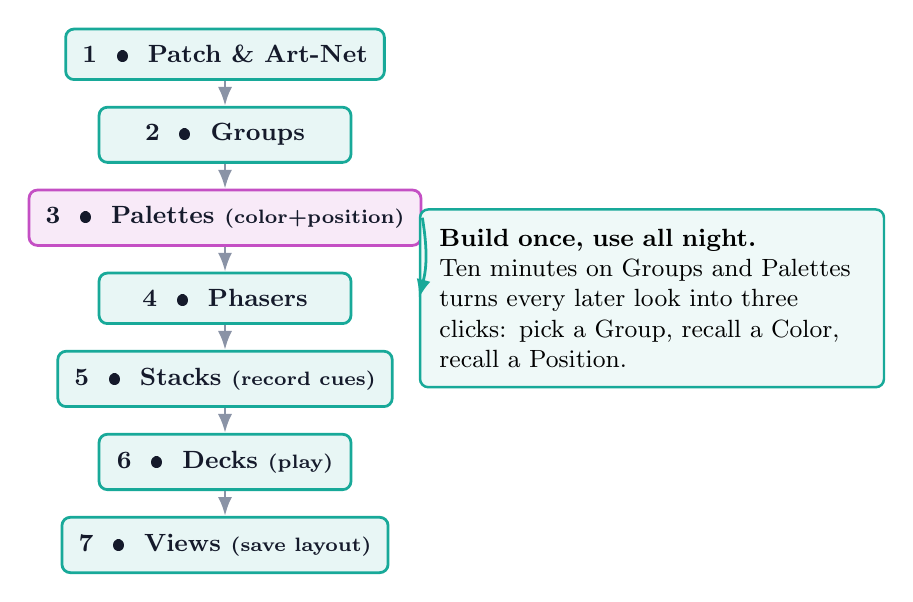
\begin{tikzpicture}[node distance=9pt, every node/.style={font=\footnotesize}]
  \node[pool,minimum width=3.2cm](s1){1 \;\textbullet\; Patch \& Art-Net};
  \node[pool,minimum width=3.2cm,below=of s1](s2){2 \;\textbullet\; Groups};
  \node[pool,minimum width=3.2cm,below=of s2,fill=cmag!12,draw=cmag](s3){3 \;\textbullet\; Palettes \scriptsize(color+position)};
  \node[pool,minimum width=3.2cm,below=of s3](s4){4 \;\textbullet\; Phasers};
  \node[pool,minimum width=3.2cm,below=of s4](s5){5 \;\textbullet\; Stacks \scriptsize(record cues)};
  \node[pool,minimum width=3.2cm,below=of s5](s6){6 \;\textbullet\; Decks \scriptsize(play)};
  \node[pool,minimum width=3.2cm,below=of s6](s7){7 \;\textbullet\; Views \scriptsize(save layout)};
  \foreach \a/\b in {s1/s2,s2/s3,s3/s4,s4/s5,s5/s6,s6/s7}{\draw[flow](\a)--(\b);}
  % side note
  \node[right=24pt of s4,box,fill=accent!7,draw=accent,text width=5.4cm,align=left](note){\textbf{Build once, use all night.}\\ Ten minutes on Groups and Palettes turns every later look into three clicks: pick a Group, recall a Color, recall a Position.};
  \draw[flow,draw=accent](s3.east) to[bend left=12] (note.west);
\end{tikzpicture}
\end{center}

% ---- WORKED EXAMPLE ------------------------------------------------------
\section{Worked example: a tiny show in 3 cues}

\begin{enumerate}[label=\textbf{\Alph*.}]
  \item \textbf{Group} --- select all movers, \badge{cmag}{Groups} $\to$ name \texttt{Movers} $\to$ Store.
  \item \textbf{Palettes} --- dial full blue $\to$ Color tab $\to$ \texttt{Blue}; dial red $\to$ \texttt{Red}. Point at the crowd $\to$ Position tab $\to$ \texttt{Audience}; point centre $\to$ \texttt{Center}.
  \item \textbf{Cue 1} --- \badge{cmag}{Stacks} $\to$ \textbf{+New} \texttt{Main}. Recall \texttt{Movers}, \texttt{Blue}, \texttt{Center}, Dimmer Full. Fade \texttt{3}s $\to$ \textbf{Store cue}.
  \item \textbf{Cue 2} --- recall \texttt{Red} + \texttt{Audience} $\to$ \textbf{Store cue}.
  \item \textbf{Cue 3} --- \badge{cmag}{Phasers} $\to$ load \texttt{Pan Sweep} $\to$ Apply $\to$ back to Stacks $\to$ \textbf{Store cue}.
  \item \textbf{Play} --- \textbf{Clear prog} (!), open \badge{cmag}{Decks}, push the \texttt{Main} fader up, press \textbf{Go} to step the cues. Pull \textbf{GM} down to dim the rig.
\end{enumerate}

\begin{tipbox}
Everything is saved to disk automatically. Reopen DMXpress and your groups,
palettes, phasers, stacks and views are all still there.
\end{tipbox}

% ---- REFERENCE -----------------------------------------------------------
\section{Reference}

\subsection{Command line}
\begin{center}\small
\rowcolors{2}{accent!5}{white}
\begin{tabularx}{\linewidth}{>{\ttfamily}l Y}
\arrayrulecolor{accent}\toprule
\rowcolor{ink}\hd{\texttt{command}} & \hd{does}\\
\midrule
clear            & Release the Programmer\\
black / bo       & Blackout --- release every stack and clear the Programmer\\
go \textnormal{[n]}   & Go on the current stack (or stack \emph{n})\\
off \textnormal{[n]}  & Release all stacks (or stack \emph{n})\\
store            & Store a cue into the current stack\\
cue n            & Jump the current stack to cue \emph{n}\\
group n          & Recall (select) group \emph{n}\\
gm n \;/\; full  & Grand Master to \emph{n}\% \;/\; 100\%\\
\bottomrule
\end{tabularx}
\end{center}

\subsection{Where your show is saved}
\begin{center}\small
\begin{tabularx}{\linewidth}{>{\ttfamily}l Y}
\arrayrulecolor{line}\toprule
\textnormal{\textbf{File}} & \textbf{Contents}\\
\midrule
groups.json   & Your Groups (saved selections)\\
palettes.json & Your Palettes (per-feature presets)\\
phasers.json  & Your Phasers (effects)\\
stacks.json   & Your Stacks and cues\\
views.json    & Your saved Views (layouts)\\
\bottomrule
\end{tabularx}
\end{center}

\vfill
\begin{center}\small\color{cgray}
The text guide lives in \texttt{GUIDE.md}. Build your Groups and Palettes first --- the rest is a few clicks.
\end{center}

\end{document}
